\section{Hardware Components and Construction}

\subsection{Cooling and air purging system}

The SVT regions are cantilevered off a chilled cold plate that is designed to remove the heat generated by the electronics and provide operational  conditions for the sensors. External cooling has been chosen over internal cooling (tubes in the modules) to keep the amount of material in the active area as low as possible. Front-end electronics is producing 5 watts per module -- 42 total modules producing 210 watts. The HFCB flex cables are routed through a 10 mm slots in the cold plate. The cold plate, (see Fig.~\ref{fig:coldplate}), includes a copper plate with brazed quarter inch copper tubes and PEEK plate on the upstream side. 

\begin{figure}[hbt] 
\centering 
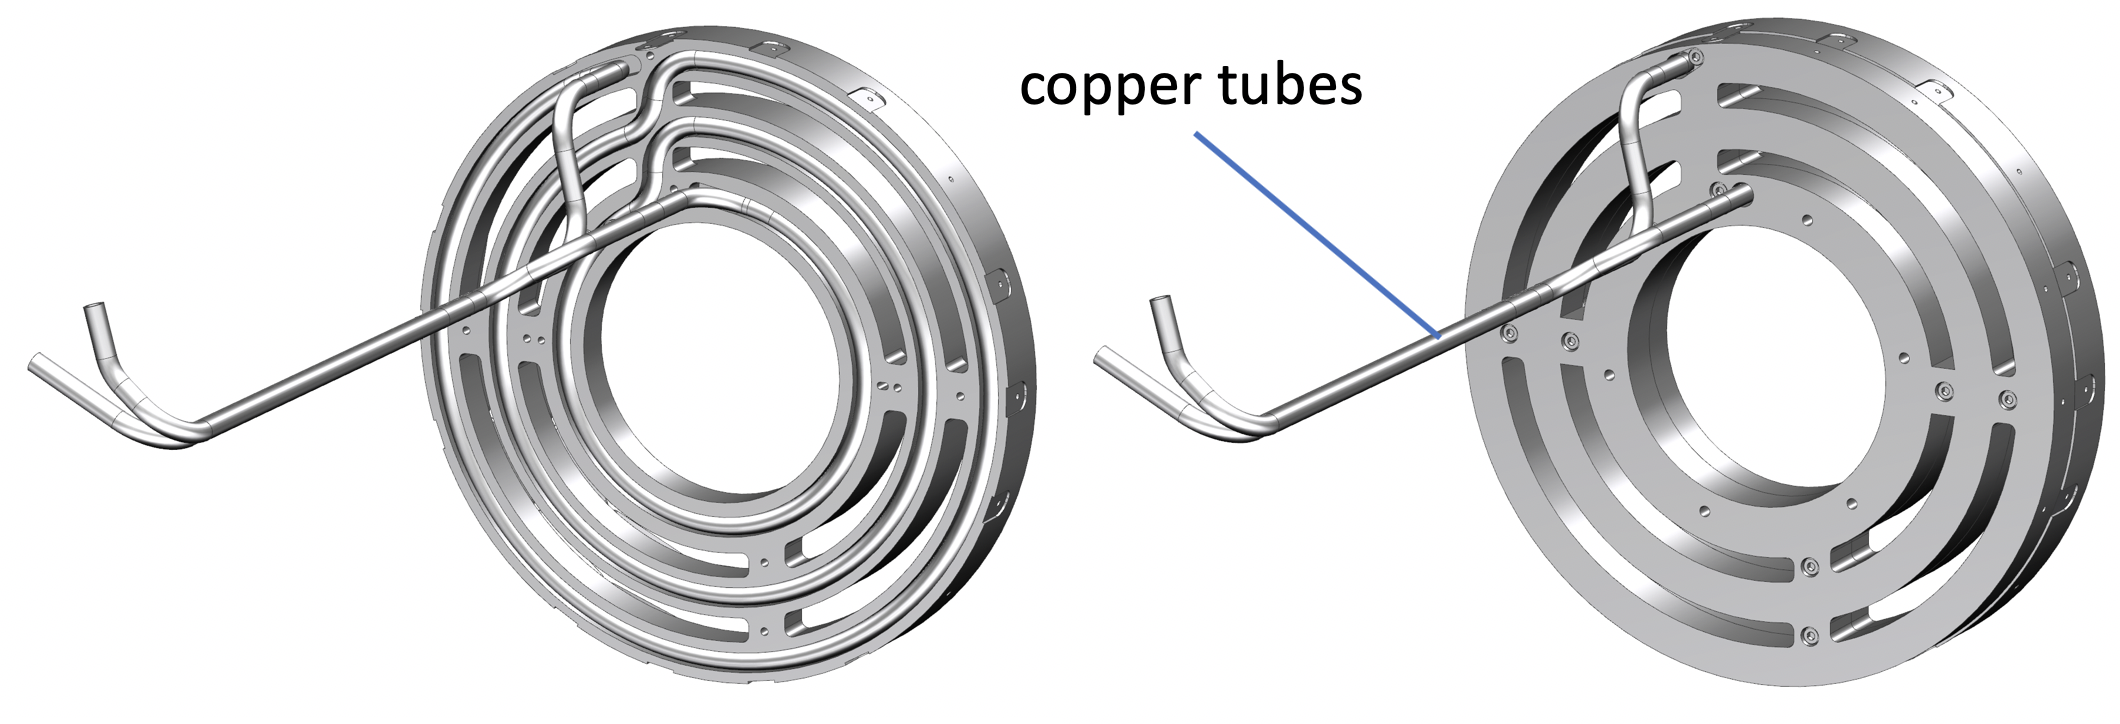
\includegraphics[width=1.0\columnwidth,keepaspectratio]{coldplate.png}
\caption{Copper tubing furnace brazed to copper cold plate (left), assembled cold plate (right).}
\label{fig:coldplate}
\end{figure}

%\begin{wrapfigure}{l}{0.5\columnwidth}
%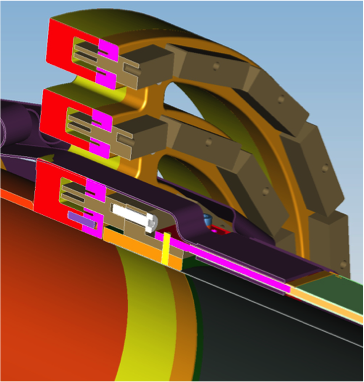
\includegraphics[width=0.5\columnwidth]{cold_plate.png}
%\caption{Routing flex cable through the cold plate.}
%\label{fig:cold-plate}
%\end{wrapfigure}

Coolant (Dynalene HC50) is flowing with a rate of 2 liters per minute at a temperature of -25$\degree$C. Cold plate upstream cover is made of PEEK plastic. Dry air flowing through the slots in the cold plate is cooled by the liquid coolant circulating in the tube inside the air purging line (see Fig.~\ref{fig:purging1}). 

\begin{figure}[hbt] 
\centering 
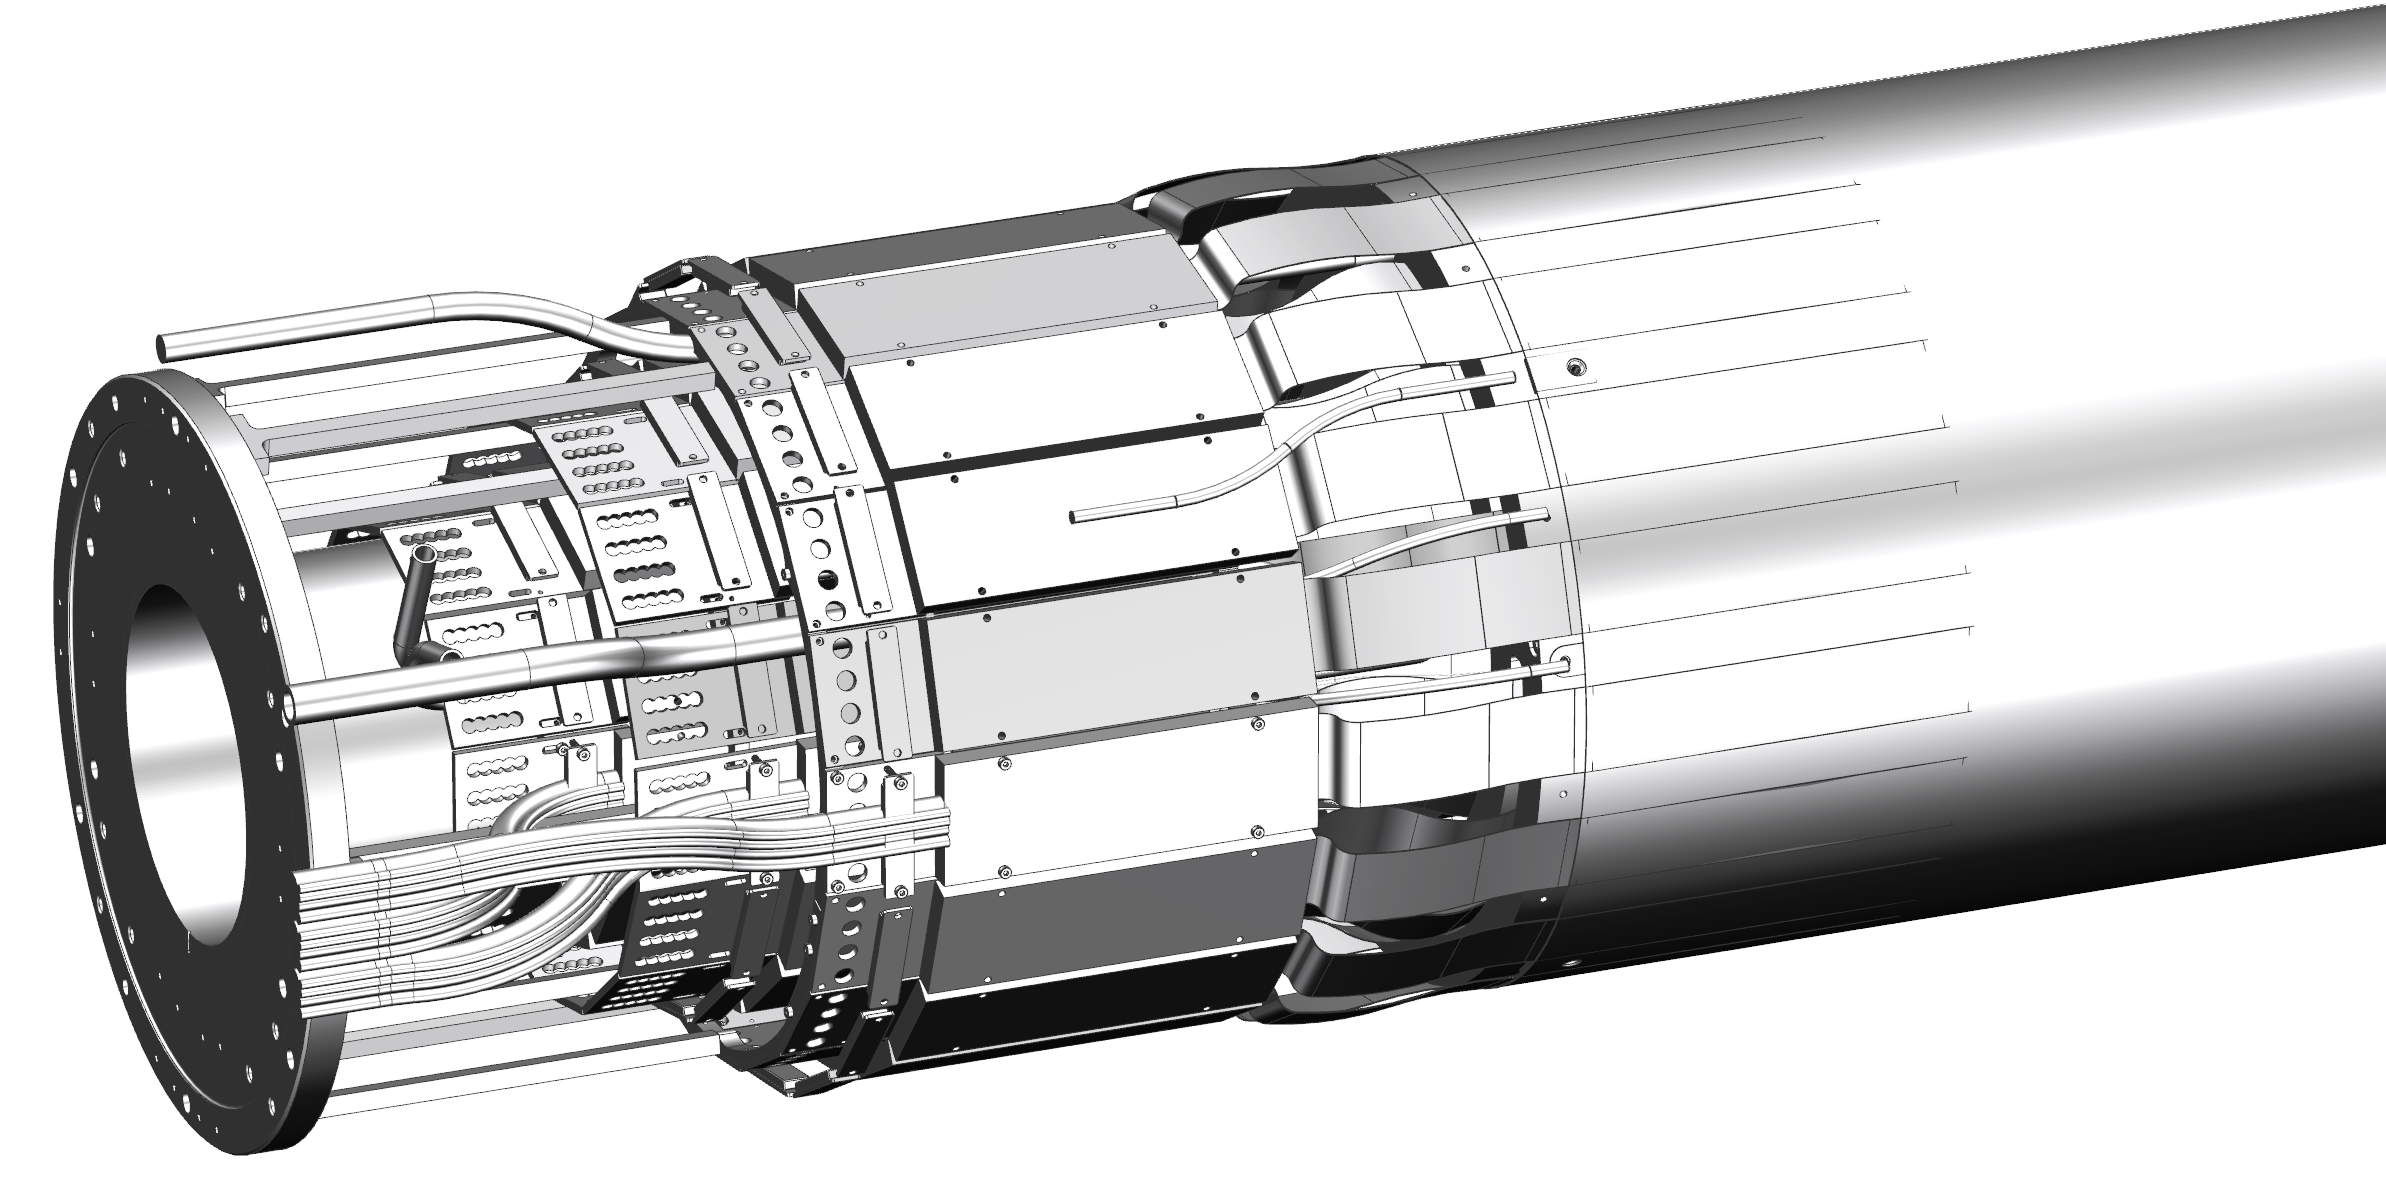
\includegraphics[width=1.0\columnwidth,keepaspectratio]{purging1.png}
\caption{Dry air flows past connectors, through the slots in the cold plate, into the Faraday cage, past sensors, and out through the holes in the cap.}
\label{fig:purging1}
\end{figure}

With 100 liters per minute of chilled air flow across the cold plate, the sensors are cooled to the operational temperature of -10$\degree$C. The Faraday cage cap on the downstream end has 4 holes to ensure the flow of cold air along the barrel. 

\begin{figure}[hbt] 
\centering 
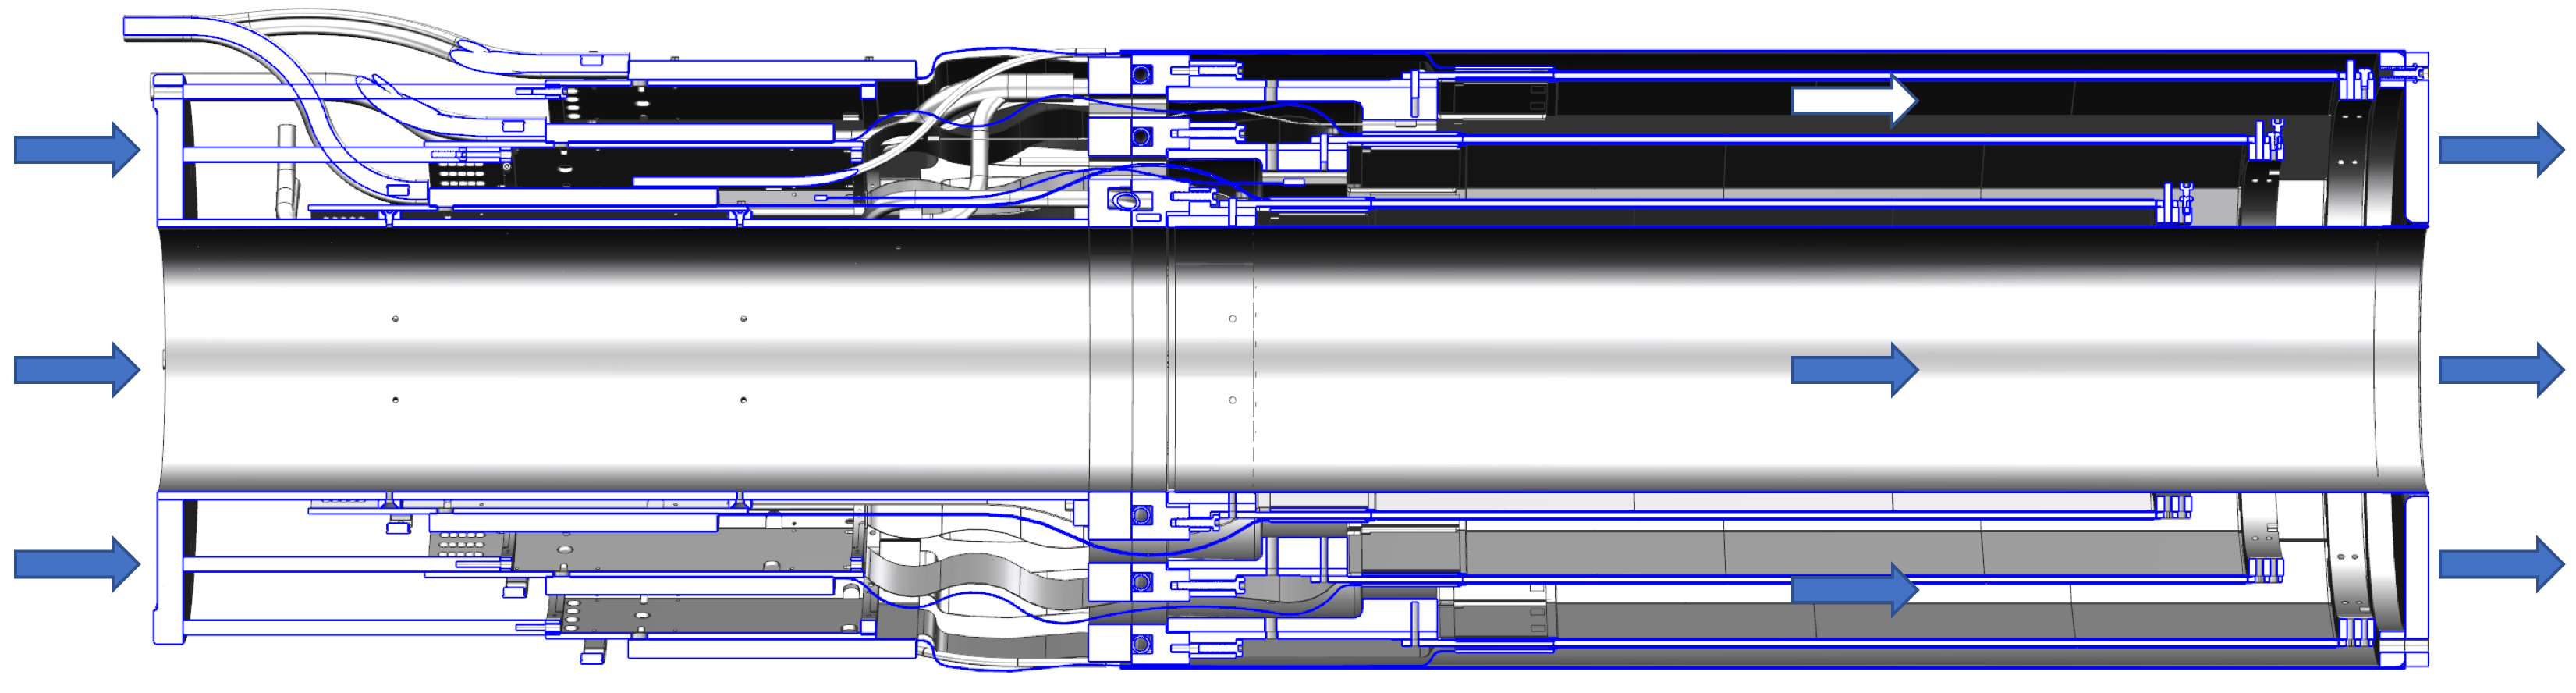
\includegraphics[width=1.0\columnwidth,keepaspectratio]{purging2.png}
\caption{Cross Section of SVT Detector.  Dry air flow in yellow.}
\label{fig:purging2}
\end{figure}

Outer shell of the Faraday cage is insulated with 3 mm thick neoprene sheet. Barrel is protected from environment humidity by purging dry air between the scattering chamber and the inner shell of the Faraday cage and between the outer shell of the Faraday cage and the protective plastic cover (see Fig.~\ref{fig:purging2}). 

\subsection{Slow controls, interlocks, and monitoring, detector safety}

Ambient conditions inside the detector are monitored by temperature and humidity sensors installed inside the downstream rings. Safe operation of the tracker is ensured by EPICS based real-time monitoring of all important operation parameters and status of hardware components. Software and hardware interlocks continuously monitor critical system parameters. The performance and stability of the system is tested at various operation temperatures. 
The SVT Hardware Interlock System (HIS) is a backup system designed to protect the detector from damage in case the main control system fails or if network communication is lost. This is a standalone system independent from the main EPICS-based slow control system and does not rely on network communications to safeguard the SVT detector. The HIS is based on the National Instruments CompactRIO (cRIO) Programmable Automation Controller (PAC) platform. cRIO is a reconfigurable embedded control and acquisition system. The cRIO system's hardware architecture includes I/O modules, a reconfigurable field-programmable gate array (FPGA) chassis, and an embedded controller. The HIS monitors key detector parameters and takes corrective action if a monitored signal is outside of pre-programmed limits. The signals monitored include: HFCB temperature, ambient and detector temperature, humidity, and dew Point, coolant flow, pressure, and temperature, coolant leak detection. Under fault conditions, the hardware interlock system disables the MPOD HV/LV crates via the front panel connector on the MPOD controller. When disabled by the HIS, the EPICS controls are overridden and all channels of the MPOD crate ramp down at their pre-programmed rate. A reset of both the HIS and the EPICS MPOD control is needed in order to re-power the HV and LV channels. Under fault conditions, the HIS shuts off the AC power to the SVT chiller via BiRa Systems Model 8880-1B1Y AC Power Module. 
TheHIS is the last line of protection for the detector. If the main EPICS slow controls system works correctly, the HIS shall never need to take corrective action to protect the detector. The trip levels for the hardware interlock system are slightly out of bounds from the EPICS trip levels to prevent both systems from tripping at the exact same level. The EPICS slow controls system (if working correctly) shall always trip first before the HIS. 
The front panel of the HIS has two interlock keys. These keys allow system experts to update the cRio system while the SVT detector is powered. These keys are normally locked in the enabled position during detector operation.
The user interface to the HIS allows the operator to remotely monitor the SVT and to set interlock trip levels. The user interface is also used to reset the system after an interlock trip event. 

Sensor leakage currents are below 400 nA with coolant at -20$\degree$C. Humidity inside the barrel is about 2~$\%$.

%\begin{figure}[hbt] 
%\centering 
%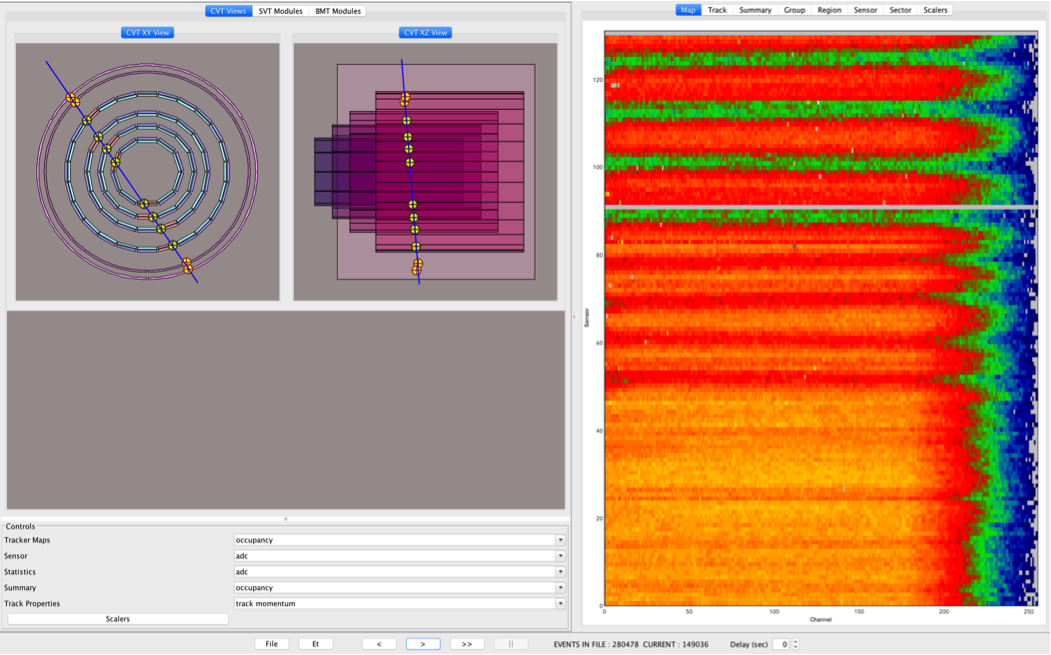
\includegraphics[width=0.9\columnwidth,keepaspectratio]{occupancy-map.png}
%\caption{Online monitoring of the SVT}
%\label{fig:monitoring}
%\end{figure}

Java based data quality monitoring tools were developed to check the quality of the data both online and offline. 
%Online SVT monitoring interface is shown in Fig.~\ref{fig:monitoring}. The tools allow the shifter to check the status of the track reconstruction and performance of the individual modules. On the left side of the interface are shown the event display and the histogram selection menus. On the right side there are canvases for the selected groups of histograms. The hit occupancy canvas is selected.

